\documentclass{mirea}

\institution{Институт искусственного интеллекта}
\faculty    {Кафедра общей информатики}
\worktype   {ОТЧЕТ \\ ПО ПРАКТИЧЕСКОЙ РАБОТЕ №12}
\workname   {Элементы алгоритмизации и процедурного программирования}
\subject    {ИНФОРМАТИКА}
\author     {Краснов Н.O.}
\examiner   {Павлова Е.С.}

\usepackage{minted}
\setminted{fontsize=\footnotesize,breaklines,baselinestretch=1}

\begin{document}

\chapter{ПОСТАНОВКА ЗАДАЧИ}
\section{Общее описание задач}
Требуется разработать блок-схему алгоритма и написать программу обработки данных. При этом требуется контролировать типы и диапазоны вводимых данных, а также предусмотреть обработку других исключительных ситуаций (если они есть), например, ситуацию деления на ноль. Блок-схема должна быть полной, т.е. должна описывать и процесс диалога с пользователем, и контроль вводимых данных, и подпрограммы вычислений с обработкой возможных исключительных операций. Блок-схема должна изображаться по ГОСТу. При обнаружении ошибки ввода или ошибки вычислений программа должна информативно уведомлять пользователя о причине ошибки. Если ошибка произошла на этапе ввода данных, то программа должна просить пользователя повторить ввод.

\section{Требования к программе}
Необходимо создать квадратную матрицу размера MxM, где M является целым числом из диапазона [2, 5]. Конкретный размер матрицы задается пользователем. Матрица содержит только целые числа из диапазона [1, 100], которые могут быть как случайными, так и вводиться пользователем. На основе созданной матрицы сделать одномерный массив, в котором сначала идут все четные элементы матрицы, упорядоченные по возрастанию, а потом идут все нечетные элементы матрицы, упорядоченные по убыванию. Результаты обработки матрицы вывести на экран.
В данной работе выполняется задание 2.9 из списка заданий в методическом указании по выполнению работ \cite[c 84]{Методичка}.

\chapter{ПРОЕКТИРОВАНИЕ И РЕАЛИЗАЦИЯ}
\section{Блок-схема программы}
На рис. \ref{fig:Блок-схема} изображена блок-схема работы программы, выполненная по Государственному стандарту ГОСТ 19.701-90 «Схемы алгоритмов программ, данных и систем» \cite{ГОСТ блок-схемы}.

\begin{figure}[ht]
	\centering
	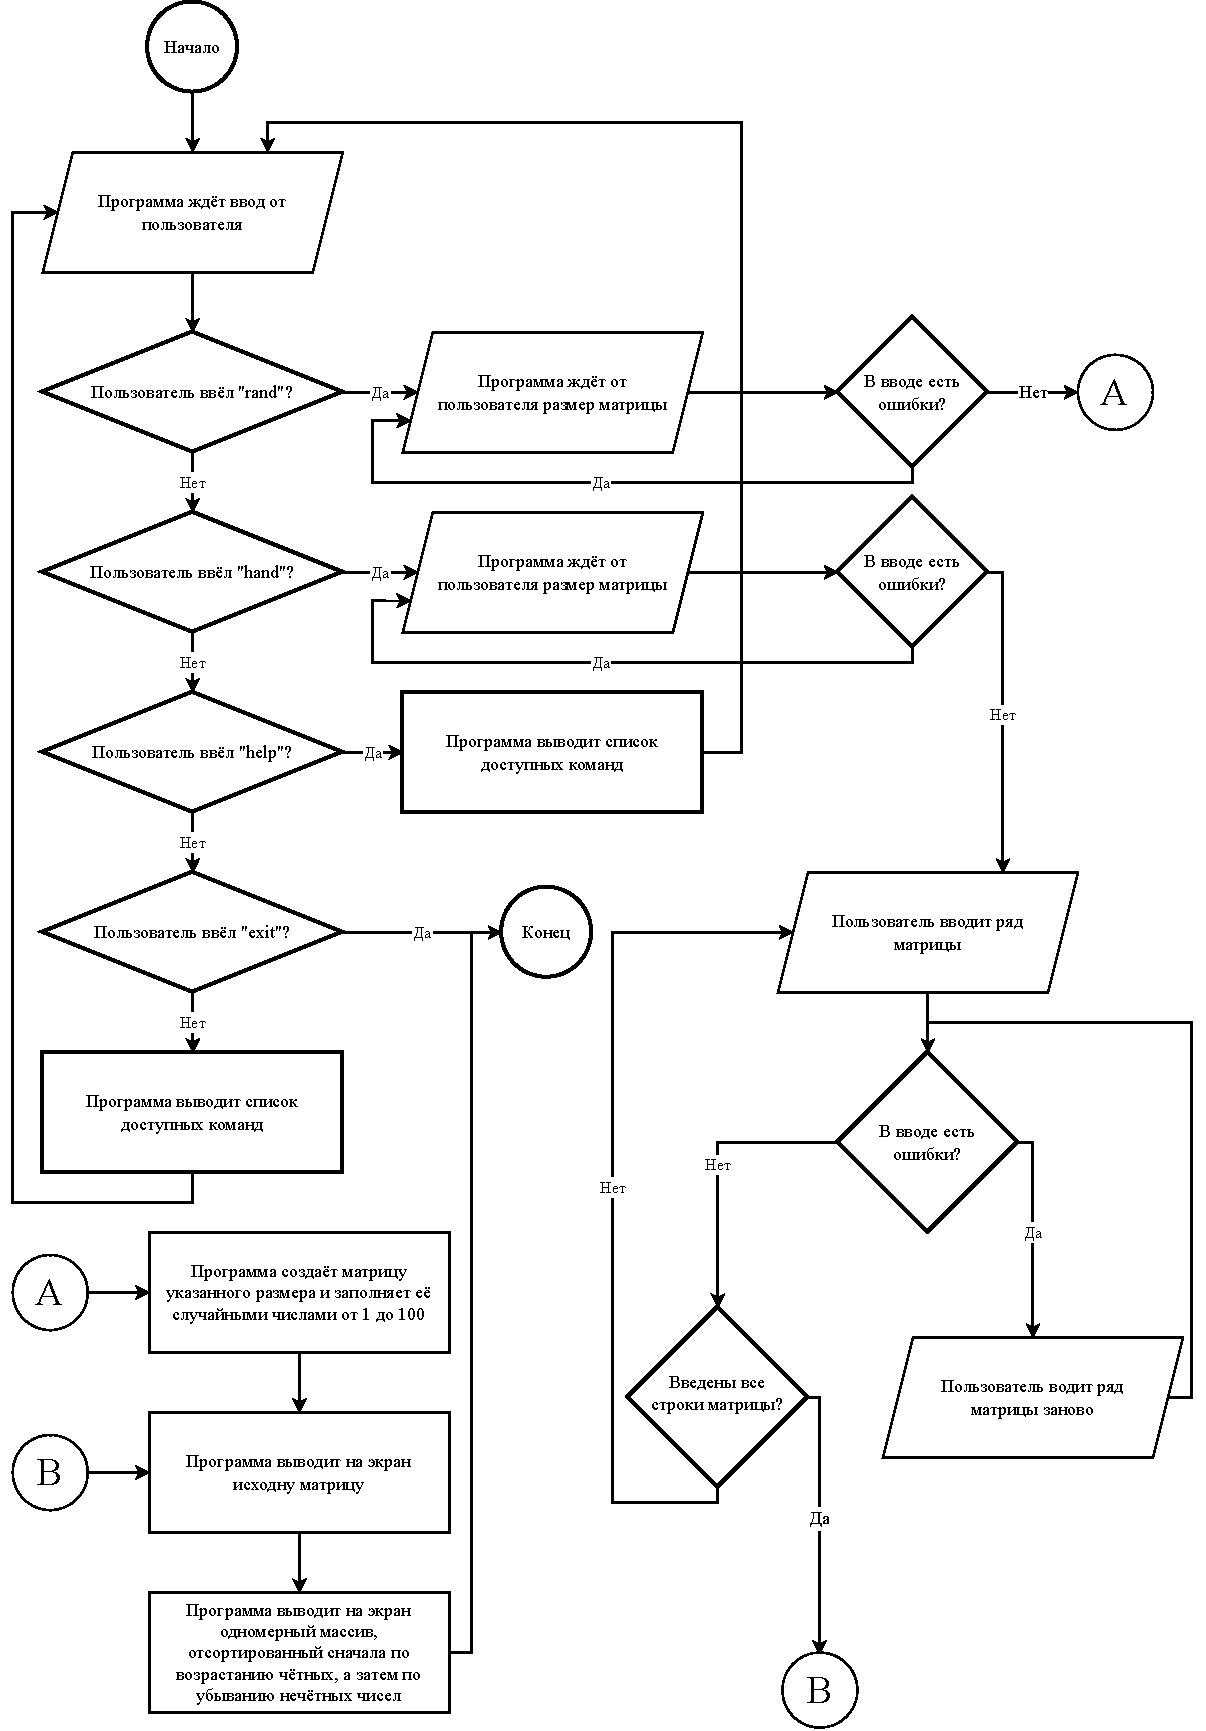
\includegraphics[width=\textwidth]{Блок-схема.pdf}
	\caption{Блок-схема работы программы}
	\label{fig:Блок-схема}
\end{figure}

\section{Структурированный код программы с комментариями}
Ниже представлены фрагменты кода программы, написанной на языке Python.

Выполнение программы начинается с функции \texttt{main}, показанной на рис. \ref{func:main}. Основываясь на вводе пользователя, отсюда вызываются все остальные подпрограммы.
\begin{figure}[ht]
	\begin{minted}{python}
def main():
 print("Напишите \"help\", чтобы узнать, что я умею!")

 while True:
     try:
         user_input = input("\n[меню]>>> ")  # Считываем ввод пользователя
     except KeyboardInterrupt:
         print()
         unknown_command()
         continue
     except EOFError:
         unknown_command()
         continue

     # Программа определяет, что ей делать, вызывая нужную функцию,
     # в зависимости от ввода пользователя
     match user_input:
         case "help":
             print_help()
         case "rand":
             random_matrix = rand_m()
             print_original_matrix_and_1d_array(random_matrix)
         case "hand":
             hand_filled_matrix = hand_m()
             print_original_matrix_and_1d_array(hand_filled_matrix)
         case "exit":
             exit()
         case _:  # Пользователь ввёл что-то неизвестное
             unknown_command()
	\end{minted}
	\caption{Функция main, точка старта программы}
	\label{func:main}
\end{figure}

Если на вход программы подается <<help>> или нечто неожиданное, что программа не способна обработать, пользователю выдается список доступных команд. За это отвечают функции \texttt{print\_help} и \texttt{unknown\_command}, показанные на рис. \ref{func:help menus}.
\begin{figure}[ht]
	\begin{minted}{python}
def print_help():
    """
    Функция print_help выводит список доступных команд,
    если хочет посмотреть меню.
    """
    print("Вот список того, что я умею")
    print("------------------------------------------------")
    print("help - Показать список доступных команд")
    print("rand - Создать квадратную матрицу c случайными числами")
    print("hand - Создать квадратную матрицу и заполнить вручную")
    print("exit - Закрыть программу")


def unknown_command():
    """
    Функция unknown_command выводит список доступных команд,
    если пользователь ошибся во вводе.
    """
    print("Неизвестная команда. Вот список того, что я умею")
    print("------------------------------------------------")
    print("help - Показать список доступных команд")
    print("rand - Создать квадратную матрицу c случайными числами")
    print("hand - Создать квадратную матрицу и заполнить вручную")
    print("exit - Закрыть программу")
	\end{minted}
	\caption{Функции, выводящие список доступных команд}
	\label{func:help menus}
\end{figure}

Функция \texttt{input\_matrix\_size}, показанная ниже, на рис. \ref{func:input size}, отвечает за обработку ввода пользователем размера необходимой ему матрицы.
\begin{figure}[ht]
	\begin{minted}{python}
def input_matrix_size():
    """
    Функция input_matrix_size просит пользователя ввести размер матрицы
    и обрабатывает ошибки при вводе.
    """
    print(
        f"Введите размер квадратной матрицы MxM, где M является целым числом "
        f"из диапазона [{SMALLEST_MATRIX_SIZE}, {BIGGEST_MATRIX_SIZE}]"
    )
    matrix_size = None
    while True:
        try:
            matrix_size = input("[размер]>>> ")
            # Пытаемся преобразовать ввод пользователя к числу. Если не
            # получается, то обрабатываем ошибку и просим заново ввести число.
            matrix_size = int(matrix_size)
            if SMALLEST_MATRIX_SIZE <= matrix_size <= BIGGEST_MATRIX_SIZE:
                break
            else:
                print(
                    f"ОШИБКА: Размер матрицы должен быть числом "
                    f"из диапазона [{SMALLEST_MATRIX_SIZE}, {BIGGEST_MATRIX_SIZE}]"
                )
                continue
        except ValueError:
            print(
                f"ОШИБКА: Размер матрицы должен быть числом "
                f"из диапазона [{SMALLEST_MATRIX_SIZE}, {BIGGEST_MATRIX_SIZE}]"
            )
            continue
        except KeyboardInterrupt:
            print()
            print("ОШИБКА: Введите размер заново")
            continue
        except EOFError:
            print("ОШИБКА: Введите размер заново")
            continue
    return matrix_size
	\end{minted}
	\caption{Функция обработки ввода размера матрицы}
	\label{func:input size}
\end{figure}

Если пользователь выбирает, что ему нужна матрица, автоматически заполненная случайными числами, вызывается подпрограмма \texttt{rand\_m}, указанная на рис. \ref{func:randm}. Основываясь на том, матрица какого размера нужна пользователю, эта функция создает двумерный массив необходимого размера и заполняет его числами от 1 до 100. Для генерации массива и заполнения его случайными числами использовалась сторонняя библиотека NumPy \cite{NymPy}.
\begin{figure}[ht]
	\begin{minted}{python}
def rand_m():
    """
    Функция rand_m отвечает за генерацию матрицы, заполненной случайными числами
    """
    matrix_size = input_matrix_size()
    # Генерируем квадратную матрицу размером matrix_size с случайными
    # числами от SMALLEST_MATRIX_ELEMENT (1) и до BIGGEST_MATRIX_ELEMENT (100)
    random_matrix = (np.random.randint(
        # Прибавляем 1 так как число берётся не включительно
        SMALLEST_MATRIX_ELEMENT,
        BIGGEST_MATRIX_ELEMENT + 1, (matrix_size, matrix_size)
    ))
    return random_matrix
	\end{minted}
	\caption{Функция, генерирующая заполненную матрицу}
	\label{func:randm}
\end{figure}

Если же пользователь выбрал, что хочет заполнить матрицу числами самостоятельно, то в программе вызывается функция \texttt{hand\_m}, показанная на рис. \ref{func:handm}.
\begin{figure}[ht]
	\begin{minted}{python}
def hand_m():
    """
    Функция hand_m обрабатывает ввод матрицы в ручном режиме.
    """
    matrix_size = input_matrix_size()
    print(
        f"Ведите через пробел элементы матрицы - целые числа в диапазоне "
        f"[{SMALLEST_MATRIX_ELEMENT}, {BIGGEST_MATRIX_ELEMENT}]: "
    )
    hand_filled_matrix = input_row_by_row(matrix_size)
    # Преобразуем вложенный массив в более удобный массив библиотеки numpy
    hand_filled_matrix = np.array(hand_filled_matrix)
    return hand_filled_matrix
	\end{minted}
	\caption{Функция для ввода матрицы вручную}
	\label{func:handm}
\end{figure}

Поскольку пользователь заполняет матрицу, вводя одну строку за другой, нам нужно что-то, что будет обрабатывать этот ввод. Для этого существует функция \texttt{input\_row\_by\_row}, представленная на рис. \ref{func:input row}.
\begin{figure}[ht]
	\begin{minted}{python}
def input_row_by_row(matrix_size):
    """
    Функция inputted_row обрабатывает ввод пользователем строк матрицы.
    """
    error_happened_during_input = False
    hand_filled_matrix = []
    print("--------начало--------")
    for row in range(matrix_size):
        while True:
            try:
                if error_happened_during_input:
                    print("--------начало--------")
                    for i in hand_filled_matrix:
                        print(*i, sep=" ")
                inputted_row = input("").split()
            except KeyboardInterrupt:
                print("ОШИБКА: Неверный ввод, попробуйте снова")
                continue
            except EOFError:
                print("ОШИБКА: Неверный ввод, попробуйте снова")
                continue
            validated_row = validate_inputted_row(inputted_row, matrix_size)
            if not validated_row:
                print("Введите строку заново")
                error_happened_during_input = True
                continue
            else:
                hand_filled_matrix.append(validated_row)
                error_happened_during_input = False
                break
    print("--------конец---------")
    return hand_filled_matrix
	\end{minted}
	\caption{Функция, отвечающая за ввод строк матрицы}
	\label{func:input row}
\end{figure}

В функции, представленной на рис. \ref{func:input row}, в свою очередь вызывается функция \texttt{validate\_inputted\_row}, которая занимается тем, что проверяет введенную пользователем строку на наличие в ней ошибок. Данная функция представлена на рис. \ref{func:validate}.
\begin{figure}[ht]
	\begin{minted}{python}
def validate_inputted_row(inputted_row, matrix_size):
    """
    Функция validate_inputted_row проверяет, являются введённые пользователем
    в строке матрицы элементы допустимыми.
    """
    try:
        validated_row = list(map(int, inputted_row))
        if len(validated_row) != matrix_size:
            print(f"ОШИБКА: В строке должно быть {matrix_size} элементов")
            return False
        for i in validated_row:
            if i > BIGGEST_MATRIX_ELEMENT or i < SMALLEST_MATRIX_ELEMENT:
                print(
                    f"ОШИБКА: Все элементы матрицы должны быть целыми числами "
                    f"в диапазоне "
                    f"[{SMALLEST_MATRIX_ELEMENT}, {BIGGEST_MATRIX_ELEMENT}]"
                )
                return
    except ValueError:
        print(
            f"ОШИБКА: Все элементы матрицы должны быть целыми числами "
            f"в диапазоне [{SMALLEST_MATRIX_ELEMENT}, {BIGGEST_MATRIX_ELEMENT}]"
        )
        return False
    return validated_row	
	\end{minted}
	\caption{Функция, проверяющая правильность ввода}
	\label{func:validate}
\end{figure}


В самом конце, необходимо вывести на экран сначала исходную матрицу, а затем эту же матрицу, представленную в виде одномерного массива, отсортированного особым образом. За это отвечает функция \texttt{print\_original\_matrix\_and\_1d\_array}, показанная на рис. \ref{func:print array}.
\begin{figure}[ht]
	\begin{minted}{python}
def print_original_matrix_and_1d_array(matrix):
    """
    Функция print_original_matrix_and_1d_array выводит в консоль сначала
    исходную матрицу, а затем матрицу, преобразованную в одномерный массив,
    отсортированный сначала по возрастанию четных элементов, а затем по убыванию
    нечётных элементов.
    """
    print()
    print("Ваша матрица:")
    print(matrix)

    # "Сплющиваем" матрицу до одномерного массива
    matrix_in_1d = list(matrix.flatten())

    even_elems = sorted(
        [num for num in matrix_in_1d if num % 2 == 0]
    )
    odd_elems = sorted(
        [num for num in matrix_in_1d if num % 2 == 1], reverse=True
    )
    print()
    print("Матрица в виде одномерного массива:")
    print([*even_elems, *odd_elems])	
	\end{minted}
	\caption{Функция для вывода на экран матрицы и одномерного массива}
	\label{func:print array}
\end{figure}

В программе также присутствуют константные значения, представленные на рис. \ref{func:constants}.
\begin{figure}[ht]
	\begin{minted}{python}
"""Константы программы"""
# Минимальный допустимый размер матрицы
SMALLEST_MATRIX_SIZE = 2
# Максимальный допустимый размер матрицы
BIGGEST_MATRIX_SIZE = 5
# Минимальный допустимый размер элементов в матрице
SMALLEST_MATRIX_ELEMENT = 1
# Максимальный допустимый размер элементов в матрице
BIGGEST_MATRIX_ELEMENT = 100
	\end{minted}
	\caption{Программные константы}
	\label{func:constants}
\end{figure}


\section{Примеры тестирования, доказывающие работоспособность}

Ниже, на рис. \ref{func:test auto}, показана работоспособность программы. В целях демонстрации отказоустойчивости программы, на её вход также были поданы неверные значения. Матрица на рис. \ref{func:test auto} была заполнена в автоматическом режиме.
\begin{figure}[ht]
	\centering
	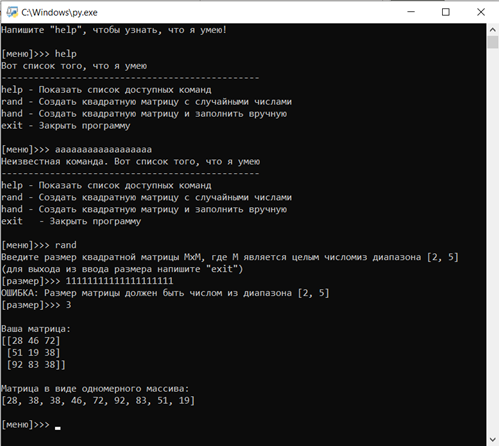
\includegraphics{Test rand.png}
	\caption{Работа программы с автозаполнением матрицы}
	\label{func:test auto}
\end{figure}

Ниже, на рис. \ref{func:test hand} показана работоспособность программы. В целях демонстрации отказоустойчивости программы, на её вход также были поданы неверные значения. Матрица на рис. \ref{func:test hand} была заполнена пользователем с клавиатуры.
\begin{figure}[ht]
	\centering
	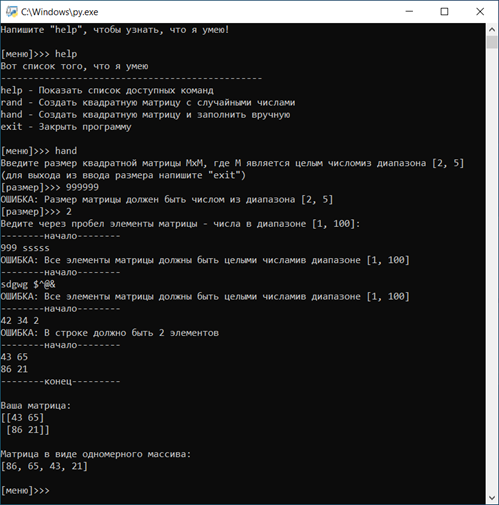
\includegraphics{Test hand.png}
	\caption{Работа программы с заполнением матрицы с клавиатуры}
	\label{func:test hand}
\end{figure}

\chapter{ВЫВОДЫ}
В ходе данной работы была разработана блок-схема, оформленная по стандарту ГОСТ. По данной схеме была разработана и многократно протестированная программа, элементы кода и работоспособность которой можно увидеть в данной работе.

\begin{thebibliography}{99}
	\bibitem{Методичка} \textbf{Смирнов, С.С.} Информатика. Методические указания по выполнению практических работ / С.С. Смирнов, Д.А. Карпов. – Москва, МИРЭА – Российский технологический университет, 2020. – 102 с.
	
	\bibitem{NymPy} NumPy : библиотека для научных вычислений с использованием Python : документация : сайт. – [Б. м.]. – URL: https://numpy.org/doc/1.23/reference/index.html (дата обращения: 29.10.2022). – Текст : электронный.
	
	\bibitem{ГОСТ блок-схемы} ГОСТ 19.701-90 Схемы алгоритмов программ, данных и систем : национальный стандарт Российской Федерации : издание официальное : утвержден и введен в действие Постановлением Государственного комитета СССР по управлению качеством продукции и стандартам от 26.12.90 № 3294 : переиздание : дата введения 1992-01-01 / разработан Государственным комитетом СССР по вычислительной технике и информатике. – Москва : Стандартинформ, 2010. – 158 c. – Текст : непосредственный.
\end{thebibliography}

\end{document}
